\subsection{ARF Rate Control Algorithm}
\label{subsec:arf}

Automatic Rate Fallback (ARF)~\cite{kamerman1997wavelan} is the first rate
control algorithm in literature. In ARF, the sender increases the bit rate after
$Th_1$ number of consecutive successes or $Th_2$ number of packets with at most
one retransmission. The sender decreases bit rate after two consecutive packet
failures or if the first packet sent after rate increase (commonly referred as
\textit{probing} packet) fails.

\sloppy{%
  Fig.~\ref{fig:arf_sm} shows the state machine $S$ for the packet trace
  collected at sender (DUT), where $\it{DATA}_i^r$ denotes a data packet
  with sequence number $i$ and bit rate $r$, $\it{DATA}_i^{r\prime}$ is a retransmission packet
  and $Ack$ is the acknowledgment packet. The \texttt{pkg\_succ} function is
  shown in Algorithm~\ref{alg:pkt_succ}.
}

\begin{figure}[t!]
  \centering
  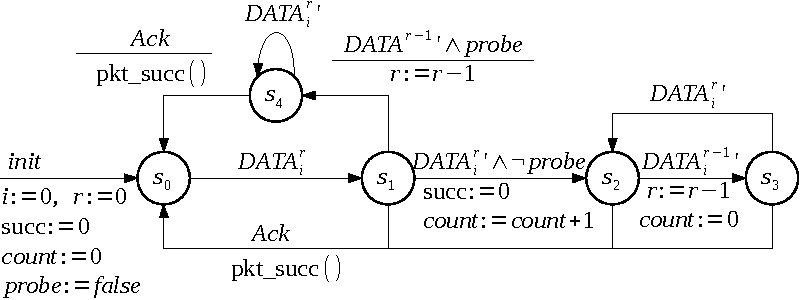
\includegraphics[width=0.8\textwidth]{arf_sm.pdf}
  \caption{\textbf{Monitor State Machine for ARF Rate Control Algorithm.} Timing
  constraints are omitted for succinctness.}
  \label{fig:arf_sm}
\end{figure}


The \texttt{succ} variable is used to track the number of consecutive packet
successes. It is increased after each packet success , and is reset to 0 after a
rate increase or upon a packet failure ($s_1\rightarrow s_2$).  Similarly,
\texttt{count} is to track the number of packets with at most one
retransmission, and is increased after packet success, or for the first packet
retransmission ($s_1\rightarrow s_2$). It is reset when there are two
consecutive packet failures ($s_2\rightarrow s_3$). Finally, the \texttt{probe}
flag is set upon rate increases to indicate the probing packet, and is cleared
upon packet success. The variable \texttt{r} is the current bit rate, which is
decreased if the probing packet fails ($s_1\rightarrow s_4$), or every two
consecutive failures ($s_2\rightarrow s_3$). If \texttt{r} is not the highest
rate, it is increased when either of the two thresholds are reached.


\begin{algorithm}[t!]
  \caption{\texttt{pkt\_succ} function}
  \label{alg:pkt_succ}
  \begin{algorithmic}[1]
    \Function{pkt\_succ}{}
    \Let{i}{(i+1)\%N}
    \Let{succ}{succ + 1}
    \Let{count}{count + 1}
    \Let{probe}{false}
    \If{r $< R$ and (succ $\ge Th_1$ or count $\ge Th_2$)}
    \Let{r}{r+1}
    \Let{succ}{0}
    \Let{count}{0}
    \Let{probe}{true}
    \EndIf
    \EndFunction
  \end{algorithmic}
\end{algorithm}

In particular, the bug we found lies in the implementation's \texttt{pkt\_succ}
function in line 6. Instead of checking \texttt{count $\ge$ Th\_2}, the
implementation checks \texttt{count == Th\_2}. This bug also exists in the NS-3
implementation of Adaptive ARF (AARF) algorithm~\cite{lacage2004ieee} and the
pseudo code implementation of AARF in~\cite{lacage2004report}.

Note that the \texttt{count} variable is incremented twice if a packet succeed
after one retransmission: once in $s_1\rightarrow s_2$, once in the
\texttt{pkt\_succ} function for the retransmission packet. Therefore, if the
value of \texttt{count} is $Th_2-1$ and the next packet succeed after one
retransmission, the value of \texttt{count} will be $Th_2+1$, which would fail
the implementation's test of \texttt{count == Th\_2}.

We report a bug found in NS-3 ARF~\cite{kamerman1997wavelan} implementation
which causes the sender to get stuck at a lower rate even after enough number of
consecutive successes. The bug was detected using sniffer traces and
confirmed by both the DUT trace and source code inspection.
